% Copyright 2006 by Till Tantau
%
% This file may be distributed and/or modified
%
% 1. under the LaTeX Project Public License and/or
% 2. under the GNU Free Documentation License.
%
% See the file doc/generic/pgf/licenses/LICENSE for more details.


\section{Shadings Library}
\label{section-library-shadings}

\begin{pgflibrary}{shadings}
  The package defines a number of shadings in addition to the ball and
  axis shadings that are available by default.
\end{pgflibrary}

In the following, the shadings defined in the library are listed in
alphabetical order. The colors of some of these shadings can be
configured using special options (like |left color|). These options
implicitly select the shading.

The three shadings |axis|, |ball|, and |radial| are always defined,
even when this library is not used.


\begin{shading}{axis}
  In this always-defined shading the colors change gradually
  between three horizontal lines. The top line is at the top
  (uppermost) point of the path, the middle is in the middle, the
  bottom line is at the bottom of the path.
  
  \begin{key}{/tikz/top color=\meta{color}}
    This option prescribes the color to be used at the top in an |axis|
    shading. When this option is given, several things happen:
    \begin{enumerate}
    \item
      The |shade| option is selected.
    \item
      The |shading=axis| option is selected.
    \item
      The middle color of the axis shading is set to the average of the
      given top color \meta{color} and of whatever color is currently
      selected for the bottom.
    \item
      The rotation angle of the shading is set to 0.
  \end{enumerate}

\begin{codeexample}[]
\tikz \draw[top color=red] (0,0) rectangle (2,1);
\end{codeexample}
  \end{key}  

  \begin{key}{/tikz/bottom color=\meta{color}}
    This option works like |top color|, only for the bottom color.
  \end{key}

  \begin{key}{/tikz/middle color=\meta{color}}
    This option specifies the color for the middle of an axis
    shading. It also sets the |shade| and |shading=axis| options, but it
    does not change the rotation angle.
    
    \emph{Note:} Since both |top color| and |bottom color| change the
    middle color, this option should be given \emph{last} if all of
    these options need to be given:
    
\begin{codeexample}[]
\tikz \draw[top color=white,bottom color=black,middle color=red]
  (0,0) rectangle (2,1);
\end{codeexample}  
  \end{key}

  \begin{key}{/tikz/left color=\meta{color}}
    This option does exactly the same as |top color|, except that the
    shading angle is set to $90^\circ$.
  \end{key}
  
  \begin{key}{/tikz/right color=\meta{color}}
    Works like |left color|.
  \end{key}
\end{shading}


\begin{shading}{ball}
  This always-defined shading fills the path with a shading that ``looks like a
  ball.'' The default ``color'' of the ball is blue (for no
  particular reason).
  
  \begin{key}{/tikz/ball color=\meta{color}}
    This option sets the color used for the ball shading. It sets the
    |shade| and |shading=ball| options. Note that the ball will never
    ``completely'' have the color \meta{color}. At its ``highlight'' spot
    a certain amount of white is mixed in, at the border a certain
    amount of black. Because of this, it also makes sense to say
    |ball color=white| or |ball color=black|
    
\begin{codeexample}[]
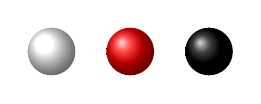
\begin{tikzpicture}
  \shade[ball color=white] (0,0) circle (2ex);
  \shade[ball color=red] (1,0) circle (2ex);
  \shade[ball color=black] (2,0) circle (2ex);
\end{tikzpicture}
\end{codeexample}
  \end{key}
\end{shading}



\begin{shading}{bilinear interpolation}
  This shading fills a rectangle with colors that a bilinearly
  interpolated between the colors in the four corners of the
  rectangle. These four colors are called |lower left|, |lower right|,
  |upper left|, and |upper right|. By changing these color, you can
  change the way the shading looks. The library also defines four
  options, called the same way, that can be used to set these colors
  and select the shading implicitly.

\begin{codeexample}[]
\tikz
  \shade[upper left=red,upper right=green,
         lower left=blue,lower right=yellow]
    (0,0) rectangle (3,2);
\end{codeexample}

  \begin{key}{/tikz/lower left=\meta{color} (initially white)}
    Sets the color to be used in a |bilinear interpolation| shading
    for the lower left corner. Also, this options selects this shading
    and sets the |shade| option.
  \end{key}

  \begin{key}{/tikz/upper left=\meta{color} (initially white)}
    Like |lower left|.
  \end{key}
  \begin{key}{/tikz/upper right=\meta{color} (initially white)}
    Like |lower left|.
  \end{key}
  \begin{key}{/tikz/lower left=\meta{color} (initially white)}
    Like |lower left|.
  \end{key}
\end{shading}


\begin{shading}{color wheel}
  \label{shading-color-wheel}
  This shading fills the path with a color wheel.
\begin{codeexample}[]
\tikz \shade[shading=color wheel] (0,0) circle (1.5);
\end{codeexample}
  To produce a color ring, cut out a circle from the color wheel:
\begin{codeexample}[]
\tikz \shade[shading=color wheel] [even odd rule]
  (0,0) circle (1.5)
  (0,0) circle (1);
\end{codeexample}
\end{shading}


\begin{shading}{color wheel black center}
  This shading looks like a color wheel, but the brightness drops to
  zero in the center.
\begin{codeexample}[]
\tikz \shade[shading=color wheel black center] (0,0) circle (1.5);
\end{codeexample}
\end{shading}


\begin{shading}{color wheel white center}
  This shading looks like a color wheel, but the saturation drops to
  zero in the center.
\begin{codeexample}[]
\tikz \shade[shading=color wheel white center] (0,0) circle (1.5);
\end{codeexample}
\end{shading}



\begin{shading}{Mandelbrot set}
  This shading is just for fun. It fills the path with a zoomable
  Mandelbrot set. Note that this is \emph{not} a bitmap
  graphic. Rather, the Mandelbrot set is \emph{computed by the
    \textsc{pdf} renderer} and can be zoomed arbitrarily (give it a
  try, if you have a fast computer).

\begin{codeexample}[]
\tikz \shade[shading=Mandelbrot set] (0,0) rectangle (2,2);
\end{codeexample}
\end{shading}



\begin{shading}{radial}
  This always-defined shading fills the path with a gradual sweep from
  a certain color in the middle to another color at the border. If the path is
  a circle, the outer color will be reached exactly at the
  border. If the shading is not a circle, the outer color will
  continue a bit towards the corners. The default inner color is
  gray, the default outer color is white.
  
  \begin{key}{/tikz/inner color=\meta{color}}
    This option sets the color used at the center of a |radial|
    shading. When this option is used, the |shade| and |shading=radial|
    options are set.
  
\begin{codeexample}[]
\tikz \draw[inner color=red] (0,0) rectangle (2,1);
\end{codeexample}
  \end{key}

  \begin{key}{/tikz/outer color=\meta{color}}
    This option sets the color used at the border and outside of a
    |radial| shading.
  
\begin{codeexample}[]
\tikz \draw[outer color=red,inner color=white]
  (0,0) rectangle (2,1);
\end{codeexample}
  \end{key}
\end{shading}


%%% Local Variables: 
%%% mode: latex
%%% TeX-master: "pgfmanual-pdftex-version"
%%% End: 
